\documentclass[times, utf8, zavrsni, numeric]{fer}
\usepackage{booktabs}
\usepackage{listings}
\usepackage{color}

\definecolor{lightgray}{rgb}{.9,.9,.9}
\definecolor{darkgray}{rgb}{.4,.4,.4}
\definecolor{purple}{rgb}{0.65, 0.12, 0.82}

\definecolor{mygreen}{rgb}{0,0.6,0}
\definecolor{mygray}{rgb}{0.5,0.5,0.5}
\definecolor{mymauve}{rgb}{0.58,0,0.82}
 
%Customize a bit the look
\lstset{ %
    backgroundcolor=\color{white}, % choose the background color; you must add \usepackage{color} or \usepackage{xcolor}
    basicstyle=\footnotesize, % the size of the fonts that are used for the code
    breakatwhitespace=false, % sets if automatic breaks should only happen at whitespace
    breaklines=true, % sets automatic line breaking
    captionpos=b, % sets the caption-position to bottom
    commentstyle=\color{mygreen}, % comment style
    deletekeywords={...}, % if you want to delete keywords from the given language
    escapeinside={\%*}{*)}, % if you want to add LaTeX within your code
    extendedchars=true, % lets you use non-ASCII characters; for 8-bits encodings only, does not work with UTF-8
    frame=single, % adds a frame around the code
    keepspaces=true, % keeps spaces in text, useful for keeping indentation of code (possibly needs columns=flexible)
    keywordstyle=\color{blue}, % keyword style
    % language=Octave, % the language of the code
    morekeywords={*,...}, % if you want to add more keywords to the set
    numbers=left, % where to put the line-numbers; possible values are (none, left, right)
    numbersep=5pt, % how far the line-numbers are from the code
    numberstyle=\tiny\color{mygray}, % the style that is used for the line-numbers
    rulecolor=\color{black}, % if not set, the frame-color may be changed on line-breaks within not-black text (e.g. comments (green here))
    showspaces=false, % show spaces everywhere adding particular underscores; it overrides 'showstringspaces'
    showstringspaces=false, % underline spaces within strings only
    showtabs=false, % show tabs within strings adding particular underscores
    stepnumber=1, % the step between two line-numbers. If it's 1, each line will be numbered
    stringstyle=\color{mymauve}, % string literal style
    tabsize=2, % sets default tabsize to 2 spaces
    title=\lstname % show the filename of files included with \lstinputlisting; also try caption instead of title
}
%END of listing package%
 
%define JavaScript language
\lstdefinelanguage{JavaScript}{
    keywords={typeof, new, true, false, function, null, var, in, let, const, class, extends, implements, constructor, super, this },
    keywordstyle=\color{black}\bfseries,  % blue
    ndkeywords={import, from, as, export, default, return, if, for, switch, while, do, else, case, break, continue},
    ndkeywordstyle=\color{black}\bfseries,  % purple
    identifierstyle=\color{black},
    sensitive=false,
    comment=[l]{//},
    morecomment=[s]{/*}{*/},
    commentstyle=\color{mygray}\ttfamily,  % green
    stringstyle=\color{darkgray}\ttfamily,  % red
    morestring=[b]',
    morestring=[b]"
}
 
\lstset{
    language=JavaScript,
    extendedchars=true,
    basicstyle=\footnotesize\ttfamily,
    showstringspaces=false,
    showspaces=false,
    numbers=left,
    numberstyle=\footnotesize,
    numbersep=9pt,
    tabsize=2,
    breaklines=true,
    showtabs=false,
    captionpos=b
}

\renewcommand{\lstlistingname}{Isječak koda}
\renewcommand{\lstlistlistingname}{Popis isječaka koda}

\newcommand{\razmakp}{\vspace{18pt}}
\newcommand{\razmaks}{\vspace{10pt}}
\newcommand{\uvlakas}{\hspace{0.5cm}}

\begin{document}

% TODO: Navedite broj rada.
\thesisnumber{5299}

% TODO: Navedite naslov rada.
\title{Korisničko sučelje knjižnice za razmjenu multimedijskog sadržaja}

% TODO: Navedite vaše ime i prezime.
\author{Petar Kovačević}

\maketitle

% Ispis stranice s napomenom o umetanju izvornika rada. Uklonite naredbu \izvornik ako želite izbaciti tu stranicu.
\izvornik

% Dodavanje zahvale ili prazne stranice. Ako ne želite dodati zahvalu, naredbu ostavite radi prazne stranice.
\zahvala{}


\tableofcontents


% Uvod
\chapter{Uvod}

Potreba za razmjenom znanja, za razmjenom iskustava i ideja je jedna od ključnih karakteristika koja čini čovjeka čovjekom.
Upravo je ta potreba, kao i sposobnost da je ispuni kvalitetnije od bilo kojeg drugog bića, snažno utjecala na evoluciju čovjeka i dovela nas na poziciji gdje se nalazimo danas.
Na poziciji vrha hranidbenog lanca i neosporivo dominantnoj vrsti na Zemlji.

Nije iznenađenje kako mnoge drevne kulture i civilizacije imaju priče u kojima nekakvo božanstvo prenosi svoje znanje ljudima.
Znanje uz pomoć kojeg ljudi postaju moćniji od svih ostalih smrtnih stvorenja.
Jedna takva priča je mit o Prometeju, titanu iz grčke mitologije koji je ukrao vatru s Olimpa i darovao je ljudima kako bi omogućio razvoj civilizacije.

\razmakp

U modernom vremenu čovjek ima gotovo neiscrpan izvor znanja.
Putem interneta može naći gotovo sve što poželi, no ipak nije sav sadržaj dospio u digitalan oblik.
To je, između ostalog, slučaj s jako specifičnim sadržajima, kao što su fakultetske skripte čija je ideja da jednostavnim jezikom sažmu i prezentiraju akademsko znanje, te sadržajima koji su na jeziku s relativno malim brojem govornika, kao što je slučaj s hrvatskim jezikom.

Jeste li ikad pokušali naći podatke na hrvatskom jeziku o nekoj knjizi, a da ona nije dio popisa za lektiru?
Jeste li ikad tražili funkcionalni primjerak videoigre izrađene u devedesetima?
Jeste li se ikad mučili s nalaženjem neke knjige koju ste htjeli pročitat?
Da je niste mogli naći u lokalnoj knjižnici ni u antikvarijatu, a u knjižarama je bila ili preskupa ili nije bila na policama, već bi se morala čekati više od mjesec dana da stigne putem narudžbe?

Vjerujem da smo se mnogi barem jednom našli u takvoj ili sličnoj situaciji.

\razmakp

Za sve te sadržaje, koje je teško naći na standardne načine, često postoji osoba koja im je vlasnik i voljna ga je posuditi.
No problem je kako naći takvu osobu, odnosno kako osobi koja je voljna nešto posuditi omogućiti da to da do znanja drugima.
\razmaks

Aplikacija čije je korisničko sučelje tema ovog rada ima za cilj riješiti upravo taj problem.

\razmakp

Ideja aplikacije je omogućiti korisnicima u hrvatskom govornom području da ponude svoje knjige, skripte, stripove, CD-ove i sl. na posuđivanje.
Odnosno, omogućiti drugim korisnicima da pronađu takav sadržaj.
Isto kao što je Prometej besebično ponudio vatru ljudima, tako korisnici aplikacije mogu drugim korisnicima ponuditi ono što imaju i time stvoriti \emph{virtualnu knjižnicu} za razmjenu multimedijskog sadržaja.

\razmakp

U ovom radu je razmotren i riješen problem izgradnje jednostavnog i interaktivnog korisničkog sučelja takve knjižnice.
Također su u radu istražene moderne tehnologije i alati za razvoj korisničkih sučelja.
Detaljno o njima se može pročitati u drugom poglavlju.
Ključna je biblioteka React opisana u potpoglavlju \ref{sec:react}.

Poslije korištenih tehnologija, u trećem poglavlju, je detaljno opisan zadatak rada te su specificirani zahtjevi, dok se opis same implementacije zadatka nalazi se u četvrtom poglavlju.
Nakon implementacije, u petom i zadnjem poglavlju, slijedi zaključak cjelokupnog rada.


% Korištene tehnologije
\chapter{Korištene tehnologije}



% ECMAScript 2015 JavaScript
\section{ECMAScript 2015 JavaScript}

Programsko rješenje je građeno primarno uz pomoć biblioteke React i pomoćnih paketa.
Jezik pisanja je JavaScript po ECMAScript 2015 (izvornog naziva ECMAScript 6, tj. ES6) specifikaciji.
Riječ je o standardu koji je uveo velike promjene u sam jezik.
U svrhu razumijevanja koda programskog rješenja, u okviru rada će se prvo ukratko razmotriti neke ključne funkcionalnosti i dodatke koje ECMAScript 2015 uvodi u JavaScript.


% Ključne riječi let i const
\subsection{Ključne riječi \emph{let} i \emph{const}}

Standardna ključna riječ za definiranje varijabli u JavaScriptu - \emph{var} ima nelogično ponašanje unutar djelokruga bloka \engl{block scope}. Promotrimo sljedeći primjer:

\razmakp
\begin{lstlisting}[language=JavaScript, caption={Primjer djelokruga \emph{var} varijable}]
function varTest() {
  var x = 1;
  if (true) {
    var x = 2;
    console.log(x);  // 2
  }
  console.log(x);  // 2
}
\end{lstlisting}
\razmaks

Varijabla definirana u \emph{if}-bloku je ista kao ona van njega, odnosno blok nije imao utjecaj na djelokrug varijable onako kako bismo očekivali u ostalim jezicima C-ovske sintakse.
\razmakp

Ovaj problem može se riješiti korištenjem ključne riječi \emph{let} umjesto \emph{var}\citep{MDNLet}.

\razmakp
\begin{lstlisting}[language=JavaScript, caption={Primjer djelokruga \emph{let} varijable}, label={lst:let_example}]
function varTest() {
  let x = 1;
  if (true) {
    let x = 2;
    console.log(x);  // 2
  }
  console.log(x);  // 1
}
\end{lstlisting}
\razmaks

Sada se dobije očekivano ponašanje. Varijabla unutar \emph{if}-bloka je nova varijabla koja je unutar svog djelokruga zasjenila varijablu u vanjskom bloku.

Također, u slučaju da se u ovom kodu (isječak koda \ref{lst:let_example}) pokušalo ponovno deklarirati varijablu \emph{x} unutar istog bloka, bila bi bačena sintaksna greška.
Varijabla deklarirana ključnom riječi \emph{var} ne baca sintaksne greške, kod nje je dopušteno redeklarirati varijable u istom bloku.
Takvo ponašanje može prouzročiti neprimjetne greške pri pisanju koda koje se teško pronalaze kasnije.

\razmakp

Još jedna razlika između \emph{var} i \emph{let} je da se u globalnom djelokrugu varijable definirane s \emph{let} ne pridružuju globalnom objektu.

\razmakp
\begin{lstlisting}[language=JavaScript, caption={Odnos \emph{var} i \emph{let} s globalnim objektom}]
var x = 'global';
let y = 'global';
console.log(this.x); // "global"
console.log(this.y); // undefined
\end{lstlisting}
\razmaks

I u ovom slučaju je ponašanje \emph{let} varijable logičnije. Samo zato što se varijabla koristi unutar neke funkcije, odnosno objekta, ne znači da je ideja tu varijablu pridružiti kao svojstvo objekta u kojem se nalazi.

\razmakp

Budući da se \emph{let} varijable ponašaju više u skladu s očekivanjem, pogotovo ako imamo podlogu u programskom jeziku koji spada u obitelj jezika C \engl{C-family programming languages}, i da bacaju iznimke u slučaju grešaka, u novijem standardu se preporuča izbjegavanje korištenja ključne riječi \emph{var} u svim situacijama.

\razmakp
\razmakp

Kako u starim verzijama nije bilo drugog načina deklariranja varijable dalje od ključne riječi \emph{var} i globalnih varijabli, programer je morao sam paziti da ne promjeni vrijednost varijabli koje si je odredio kao konstante
U novom standardu je taj problem riješen ključnom riječi \emph{const}\citep{MDNConst}.

\razmakp
\begin{lstlisting}[language=JavaScript, caption={Deklariranje konstante}]
const PI = 3.14
PI = 3  // error
\end{lstlisting}
\razmaks

Po pitanju djelokruga, ponašanje konstanti je identično ponašanju \emph{let} varijable.

\razmakp


% Klase i nasljeđivanje
\subsection{Klase i nasljeđivanje}

Glavna novost u ECMAScript 2015 je uvođenje klasa.
Prethodno se nasljeđivanje u JavaScriptu ostvarivalo kreiranjem objekata iz postojećih objekata te dodavanju novih metoda i atributa novostvorenom objektu.
Odnosno svaki objekt u JavaScriptu ima skriveno svojstvo prototip \engl{prototype} koje sadrži poveznicu do nekog drugog objekta, putem kojeg možemo ostvariti nasljeđiavnje\citep{MDNPrototype}.
Takva mehanika je puno moćnija od korištenja klasa, odnosno nudi puno više fleksibilnosti, no istovremeno uzrokuje puno nejasniju strukturu koda.

Klase u novom standardu su ostvarene kao poseban oblik funkcija\citep{MDNClass}.
Oba se objekta deklariraju i rukuju na identičan način, samo za različite svrhe.
Pri prevođenju JavaScripta pisanog u novom standardu u stariji (zbog kompatibilnosti sa starijim preglednicima) klase se prevode u funkcije.
(Primjer: isječak koda \ref{lst:class_example_old_js} - izrađen putem prevoditelja Babel\footnote{\url{https://babeljs.io}}).

\razmakp
\begin{lstlisting}[language=JavaScript, caption={Primjer klase}, label={lst:class_example}]
class Rectangle {
  constructor(height, width) {
    this.height = height;
    this.width = width;
  }
}
\end{lstlisting}
\razmaks

\razmakp
\begin{lstlisting}[language=JavaScript, caption={Isječak koda \ref{lst:class_example} preveden u stari standard}, label={lst:class_example_old_js}]
function _classCallCheck(instance, Constructor) {
  if (!(instance instanceof Constructor)) {
    throw new TypeError("Cannot call a class as a function");
  }
}

var Rectangle = function Rectangle(height, width) {
  _classCallCheck(this, Rectangle);

  this.height = height;
  this.width = width;
};
\end{lstlisting}
\razmaks

Nasljeđivanje klasa postiže se sintaksom sličnom programskom jeziku Java.
Ključna riječ kojom se definira nasljeđivanje je \emph{extends}, dok se nadklasa poziva s ključnom riječi \emph{super}.

\razmakp
\begin{lstlisting}[language=JavaScript, caption={Primjer naljeđivanja}]
class Cat { 
  constructor(name) {
    this.name = name;
  }
  speak() {
    console.log(this.name + ' makes a noise.');
  }
}

class Lion extends Cat {
  speak() {
    super.speak();
    console.log(this.name + ' roars.');
  }
}

let l = new Lion('Simba');
l.speak(); 
// Simba makes a noise.
// Simba roars.
\end{lstlisting}
\razmaks


% Promise objekt
\subsection{\emph{Promise} objekt} \label{sec:promise}

Obećanje \engl{Promise} je poseban objekt koji predstavlja izvršavanje asinkrone operacije.
Ideja je da se neka asinkrona operacija (npr. dohvat podataka s poslužitelja) omota u obećanje kako bi se definiralo što će se izvršiti u slučaju uspjeha ili neuspjeha.
Operacija koja se izvršava nakon obećanja može ponovno biti obećanje.
To nizanje obećanja \engl{chaining}, koje se ostvaruje putem funkcije \emph{then}, je zgodno rješenje kada logika zahtjeva višestruko ugnježđivanje funkcija povratnog poziva \engl{callback function}\citep{MDNUsingPromises}.
Primjer toga je u sljedećem isječku koda (\ref{lst:callback_vs_promises})

\razmakp
\begin{lstlisting}[language=JavaScript, caption={Korištenje obećanja umjesto ugnježđivanja funkcija povratnog poziva}, label={lst:callback_vs_promises}]
// callback pyramid of doom
doSomething(function(result) {
  doSomethingElse(result, function(newResult) {
    doThirdThing(newResult, function(finalResult) {
      console.log('Got the final result: ' + finalResult);
    }, failureCallback);
  }, failureCallback);
}, failureCallback);

// using promises
doSomething()
.then(function(result) {
  return doSomethingElse(result);
})
.then(function(newResult) {
  return doThirdThing(newResult);
})
.then(function(finalResult) {
  console.log('Got the final result: ' + finalResult);
})
.catch(failureCallback);
\end{lstlisting}
\razmaks

Životni ciklus objekta obećanja možemo pojednostavljeno opisati dijagramom na slici \ref{fig:promise_lifecycle}.
Kada se objekt stvori, on je u stanju iščekivanja \engl{pending}.
Ovisno o uspješnosti operacije prelazi u stanja \emph{ispunjen} \engl{fufilled} ili \emph{odbačen} \engl{rejected}.
Iz tih stanja može vratiti neku povratnu vrijednost koja se onda omata kao novo obećanje.

\begin{figure}[htb]
\centering
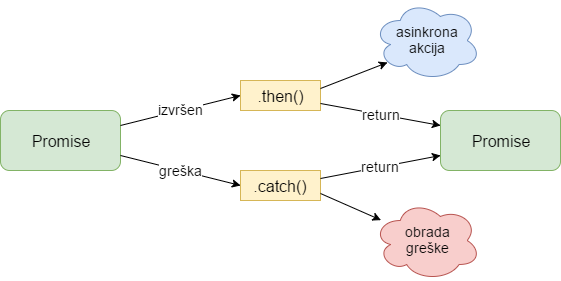
\includegraphics[width=14cm]{img/promise.png}
\caption{Životni ciklus \emph{promise} objekta}
\label{fig:promise_lifecycle}
\end{figure}

\razmakp


% Arrow funkcije
\subsection{\emph{Arrow} funkcije}

Novim standardom je u JavaScript dodano mnogo \emph{sintaksnog šećera} \engl{syntax sugars}, jedna od kojih su i funkcije napisane sa strelicom \engl{arrow functions}.
Riječ je o kraćem načinu za zapisivati anonimne funkcije po uzoru na lambda račun.

\razmakp
\begin{lstlisting}[language=JavaScript, caption={Kod iz isječka \ref{lst:callback_vs_promises} napisan pomoću \emph{arrow} funkcija}, label={lst:arrow_promises}]
doSomething()
.then(result => doSomethingElse(result))
.then(newResult => doThirdThing(newResult))
.then(finalResult => {
  console.log('Got the final result: ' + finalResult);
})
.catch(failureCallback);
\end{lstlisting}
\razmaks

Na prvi pogled ništa novo, samo kraći zapis postojeće funkcionalnosti, no \emph{arrow} funkcije nisu u potpunosti ekvivalentne već postojećim anonimnim funkcijama u JavaScriptu.
Unutar tijela starih anonimnih funkcija, referenca \emph{this} se odnosila na okolinu, tj. objekt kojem je funkcija pridružena, a ne gdje je definirana.
To je zahtjevalo dodatnu pažnju programera pri baratanju tom ključnom riječi.
\emph{Arrow} funkcije ne pate od tog problema, one ne mijenjaju referencu \emph{this} pri stvaranju novog objekta funkcije, već pozivaju \emph{this} u kojem su definirane\citep{MDNArrowFunc}.

\razmakp

\razmakp
\begin{lstlisting}[language=JavaScript, caption={Ponašanje ključne riječi \emph{this} u obe verzije anonimnih funkcija}]
function Object1(){
  this.log = function() {
    console.log(this);
  };
}
function Object2(message){
  this.log = () => console.log(this);
}

var o1 = new Object1();
o1.log()  // Object1
var method1 = o1.log;
method1();  // Window

var o2 = new Object2();
o2.log()  // Object2
var method2 = o2.log;
method2();  // Object2
\end{lstlisting}
\razmaks

\newpage


% React
\section{React} \label{sec:react}

React je JavaScript biblioteka otvorenog koda namijenjena brzoj i jednostavnoj izgradnji korisničkog sučelja. Razvijena je od strane Facebooka 2013.\ godine i zadnja stabilna verzija u trenutku pisanja ovog rada je 15.5.4.\citep{reactWiki}.
U izvorima se biblioteka također može naći pod nazivima \emph{React.js} i \emph{ReactJS}, dok je React Native radni okvir za razvoj mobilnih aplikacija u JavaScriptu na sličan način kako se web aplikacije grade u Reactu.

Bitno je za naglasiti da, iako je React biblioteka \engl{library}, nije u potpunosti netočno zvati je radnim okvirom \engl{framework}.
Tokom vremena nagomilalo se mnoštvo biblioteka i radnih okvira za korištenje sa samim Reactom, da se pod izrazom \glqq React\grqq često podrazumijeva i njihovo korištenje, što daje dojam cjelokupnog radnog okvira.
No, po svojoj definiciji je biblioteka\citep{reactGithub}.

\razmakp

Reactom se grade jednostranične \engl{single page} web aplikacije.
Produkcijska verzija React stranice se često sastoji od jedne male HTML datoteke (reda veličine dvadesetak linija koda) i JavaScript datoteke od nekoliko desetaka tisuća linija koda\footnote{Tijekom razvoja je kod u više datoteka koje se zapakiraju u jednu pri gradnji produkcijske verzije.}.
Razlog tomu je što je sav sadržaj stranice ugrađen u JavaScript kako bi se mogao dinamički mijenjati.

React koristi virtualni DOM \engl{virtual DOM\footnote{krat. \emph{Document Object Model}}}.
Virtualni DOM je apstrakcija standardnog HTML DOM-a koja se koristi kako bi se izbjegle skupe operacije dodavanja i brisanja elemenata u DOM-u.
Efikasnim upravljanjem virtualnim DOM-om, elementi se crtaju u stvarni DOM samo kada je to potrebno, odnosno crtaju se samo elementi koji su se promijenili.
Primjerice, nepotrebno je da se svaki put iznova crta (odnosno iščitava iz HTML dokumenta) navigacija, ako se samo mijenja sadržaj ispod nje.

\razmakp


% Komponente
\subsection{Komponente} \label{sec:components}

Filozofija Reacta je rastaviti korisničko sučelje na komponente kao izolirane cjeline koje se mogu ponovno upotrijebiti\citep{react}.
Instance komponenti se, slično HTML DOM elementima, organiziraju u stablastu strukturu.
Za razliku od DOM elemenata, komponente imaju vlastito stanje i logiku.
React komponente nasljeđuju klasu \emph{React.Component} te obavezno implementiraju \emph{render} metodu koja vraća React element, odnosno stablo React elemenata\citep{reactDocsComponent}.
React elementi su nepromjenjivi objekti čije je stvaranje jeftina operacija.
Crtaju se kao elementi DOM-a po potrebi\citep{reactDocsRenderElem}.

\razmakp
\begin{lstlisting}[language=JavaScript, caption={Primjer komponente}, label={lst:component_example}]
class HelloWorld extends React.Component {
  render() {
    return <h1>Hello world!</h1>;
  }
}
\end{lstlisting}
\razmaks

Osim metode \emph{render}, komponenta može implementirati vlastite metode i nadjačati metode nadrazreda (\emph{React.Component}), tj. metode životnog ciklusa \engl{lifecycle methods}.
Metode životnog ciklusa dijelimo na tri skupine:
\begin{enumerate}
  \item \emph{Mounting} -- Metode koje se pozivaju kada se stvara instanca komponente i dodaje DOM-u.
  \begin{itemize}
    \item \emph{constructor()}
    \item \emph{componentWillMount()}
    \item \emph{render()}
    \item \emph{componentDiDMount()}
  \end{itemize}
  \item \emph{Updating} -- Metode koje se pozivaju kada se dogodi promjena stanja komponente i mora se ponovno crtati u DOM-u.
  \begin{itemize}
    \item \emph{componentWillReceiveProps()}
    \item \emph{shouldComponentUpdate()}
    \item \emph{componentWillUpdate()}
    \item \emph{render()}
    \item \emph{componentDidUpdate()}
  \end{itemize}
  \item \emph{Unmounting} -- Metode koje se pozivaju kada se komponenta uklanja iz DOM-a.
  \begin{itemize}
    \item \emph{componentWillUnmount()}
  \end{itemize}
\end{enumerate}
\razmaks

Metode se pozivaju redoslijedom kojim su napisane, a uz njih se još nasljeđuju metode \emph{setState}
i \emph{forceUpdate()}.
One nisu dio životnog ciklusa, već se pozivaju nad objektom.

Svaka od metoda životnog ciklusa ima različito ponašanje, stoga postoje dobre prakse za što se koja od njih koristi.
Metoda \emph{constructor} se koristi za inicijaliziranje stanja, dok se logika promjene stanja preporučuje pisati u \emph{componentDiDMount}.\footnote{Dohvat podataka sa servera se često vrši u \emph{componentDiDMount}. Ti se podaci potom spremaju u stanje kako bi se izazvalo ponovno pozivanje metode \emph{render}.}
Razlog tomu je što promjena stanja u \emph{componentDiDMount} izaziva ponovno crtanje komponente u DOM-u, odnosno poziv metode \emph{render}.
Stanje se mijenja pozivanjem metode \emph{setState} nad objektom komponente (\glqq \emph{this.setState()}\grqq ).
Ta metoda je asinkrona, stoga promjena stanja ne blokira daljnje pozive metoda u životnom ciklusu.
Ponovno crtanje može se izbjeći ako se metodu \emph{shouldComponentUpdate} postavi da vraća \emph{false}.
U tom slučaju ponovno crtanje komponente može se postići samo pozivanjem metode \emph{force update}.

\razmakp
\razmakp

Uz stanje postoji još jedno ugrađeno svojstvo komponente, a to je \emph{props}\citep{reactDocsComp&Props}.
Ono se koristi kao objekt putem kojeg se predaju argumenti iz više komponente u nižu.
Primjer takvog korištenja je komponenta koja sadrži listu drugih komponenti, a treba odrediti nazive i ključeve potkomponenti.
U tom slučaju se, pri stvaranju potkomponenti kojima se nadjačava konstruktor, mora paziti da se koristi oblik konstruktora kakav je prikazan u isječku koda \ref{lst:component_props_example}.
Ako se ne definira vlastiti konstruktor, taj oblik konstruktora nasljeđuje se iz nadklase.\footnote{U isječku koda \ref{lst:component_props_example} je pisanje konstruktora nepotrebno.}

\razmakp
\begin{lstlisting}[language=JavaScript, caption={Primjer komponente s \emph{props}}, label={lst:component_props_example}]
class Welcome extends React.Component {
  constructor(props) {
    super(props)
  }

  render() {
    return <h1>Hello, {this.props.name}</h1>;
  }
}
\end{lstlisting}
\razmaks

Svojstva se pridodaju objektu \emph{props} iz nadkomponente na način kako je prikazano u isječku koda \ref{lst:component_sending_props}.
Pojašnjenje sintakse može se pronaći u pododjeljku \ref{sec:jsx}.

\razmakp
\begin{lstlisting}[language=JavaScript, caption={Primjer korištenja \emph{props}}, label={lst:component_sending_props}]
class Welcome extends React.Component {
  render() {
    return <h1>Hello, {this.props.name}</h1>;
  }
}

class App extends React.Component {
  render () {
    return (
      <div>
        <Welcome name="Ed" />
        <Welcome name="Edd" />
        <Welcome name="Eddy" />
      </div>
    );
  }
}
\end{lstlisting}
\razmaks


% JSX
\subsection{JSX} \label{sec:jsx}

JSX je sintaksno proširenje JavaScripta koji omogućuje jednostavno stvaranje React elemenata u formatu sličnom HTML-u.
Datoteke koje koriste ovo sintaksno proširenje se često pišu s ekstenzijom \glqq \emph{ .jsx}\grqq , no pisanje te ekstenzije nije nužno.\footnote{Za TypeScript datoteke: \glqq \emph{ .tsx}\grqq }

\razmakp

U isječku koda \ref{lst:component_sending_props} \emph{render} metoda komponente \emph{App} vraća tri instance komponente \emph{Welcome} ugnježđene u \emph{div}.\footnote{U metodi \emph{render} sve korištene komponente uvijek moraju biti ugnjeđene u jednu vršnu komponentu.}
Argumenti koji se predaju kao svojstva objekta \emph{props} pri stvaranju React elementa se pišu kao atributi DOM elemenata.
Budući da se u ovoj sintaksi React elementi mogu kombinirati s HTML elementima, pravilo je da se React elementi pišu velikim početnim slovom\citep{reactDocsJSX}.

Ovakav format daje čitku strukturu kako će se React elementi posložiti u DOM-u.
Primjerice, poziv metode \emph{render} iz klase \emph{App} bi rezultirao stvaranjem HTML koda kao u isječku \ref{lst:elements_html}.

\razmakp
\begin{lstlisting}[language=html, caption={Elementi isječka koda \ref{lst:component_sending_props} prikazani kao renderirani DOM elementi}, label={lst:elements_html}]
<div>
  <h1>Hello, Ed</h1>
  <h1>Hello, Edd</h1>
  <h1>Hello, Eddy</h1>
</div>
\end{lstlisting}
\razmaks

Kako su u JavaScriptu klase samo poseban oblik funkcija, JSX sintaksa omogućava da se jednostavne elemente stvori pomoću anonimnih funkcija.
Funkcije mogu primati proizvoljan broj argumenata, a vraćaju React element.
Elementi se imenuju tako da te funkcije spreme u varijable, odnosno konstante, koje se potom koriste isto kao i komponente.

\razmakp
\begin{lstlisting}[language=JavaScript, caption={Korištenje anonimne funkcije za stvaranje elementa}]
class App extends React.Component {
  render () {
    const Welcome = (props) => <h1>Hello, {props.name}</h1>;
    
    return (
      <div>
        <Welcome name="Ed" />
        <Welcome name="Edd" />
        <Welcome name="Eddy" />
      </div>
    );
  }
}
\end{lstlisting}
\razmaks

U svim primjerima dosad se vrijednosti dohvaćalo tako da ih se zapisivalo unutar vitičastih zagrada.
Ta sintaksa vitičastih zagrada se može iskoristiti i za istinosne vrijednosti, pomoću kojih se može \emph{short-circut} evaluacijom logičkih izraza ostvariti crtanje elementa ovisno o nekom uvjetu.

\razmakp
\begin{lstlisting}[language=JavaScript, caption={Uvjetno crtanje elementa}]
class App extends React.Component {
  render () {
    const Message = (props) => <h1>Ja sam {props.msg}</h1>;
    let f = true;
    
    return (
      <div>
        {f && <Message msg="vidljiv" /> }
        {!f && <Message msg="nevidljiv" /> }
        {!f || <Message msg="vidljiv" /> }
        {f || <Message msg="nevidljiv" /> }
      </div>
    );
  }
}
\end{lstlisting}
\razmaks


% Podizanje stanja
\subsection{Podizanje stanja} \label{sec:lifting_state}

U interaktivnoj aplikaciji često je potrebno na promjenu jednog elementa mijenjati drugi.
Primjerice, na unos teksta u okvir za pretraživanje filtrirati retke tablice s obzirom na neku od vrijednosti.
U Reactu se ta funkcionalnost postiže podizanjem stanja\citep{reactDocsLiftStateUp}.

Na istom tom primjeru, ako su komponente okvira za unost teksta i tablice ugniježđene u zajedničkoj roditeljskoj komponenti, vrijednost teksta koji se unosi i lista s podacima za retke tablice bi se definirali kao atributi stanja te roditeljske komponente.
Ugniježđene komponente bi putem \emph{props} primile te atribute iz roditeljske komponente.
Pri tome, komponenta koja uzrokuje promjenu stanja, što je u ovom slučaju komponenta u koju se unosi tekst, mora primiti i referencu na funkciju koju će pozvati kad se unos promijeni.
Ta funkcija se nalazi u roditeljskoj komponenti i postavlja stanje na novu vrijednost, što uzrokuje ponovno crtanje ugniježđenih elemenata, odnosno komponenti.
Na taj način se komponenta s tablicom može svaki put crtati s filtriranom listom redaka, s obzirom na uneseni tekst.

Reactova hijerarhija komponenti prati filozofiju \glqq Podaci dolje, akcije gore\grqq \break \engl{Data Down, Actions Up}.
U opisanom primjeru su podaci vrijednosti koje se šalju elementima, dok je akcija poziv funkcije roditeljske komponente koja mijenja stanje.

\newpage


% Paket create-react-app
\section{Paket \emph{create-react-app}}

Npm\footnote{Upravitelj paketa za JavaScript, primarno korišten uz Node.js.} paket \emph{create-react-app} omogućuje stvaranje podešene React aplikacije, u svrhu bržeg i lakšeg razvoja nove aplikacije.
Aplikacija stvorena ovim paketom ima podešen prevoditelj \emph{Babel}\footnote{Prevodi novije JavaScript funkcionalnosti u stari standard, \url{http://babeljs.io} }, upravitelj modulima \emph{webpack}\footnote{Sažima sve module i pakete o kojima ovise u statičke resurse, \url{https://webpack.github.io} } i mnoge druge dodatke koji su često potrebni u razvoju React aplikacija\citep{createReactAppGithub}.
Podešene su također i skripte za pokretanje, testiranje i izradu produkcijske verzije.

Sve te postavke su skrivene, a programer nakon stvaranja aplikacije vidi strukturu kao u slici \ref{fig:app-structure}.\footnote{Mapa novostvorene aplikacije na disku zauzima prostor od otprilike 100 MB.}
U slučaju potrebe za promjenom predefiniranih postavki pokreće se skripta \glqq \emph{npm run eject}\grqq ~ koja nepovratno otkriva sve konfiguracijske datoteke.

\razmaks

\begin{figure}[htb]
\centering
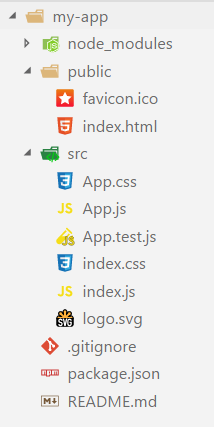
\includegraphics[width=6cm]{img/app-structure.png}
\caption{Struktura aplikacije stvorene pomoću \emph{create-react-app}}
\label{fig:app-structure}
\end{figure}

\newpage


% Paket react-router
\section{Paket \emph{react-router}} \label{sec:react-router}

Pri gradnji jednostraničnioh web aplikacija, često nije u cilju da se korisniku doimaju kao takve.
Korisnik želi imati mogućnosti da putem poveznice izravno dođe do nekog dijela aplikacije ili da se vrati na prethodno stanje aplikacije klikom \emph{Nazad} u pregledniku, kao što to može s klasičnim web stranicama.\footnote{Ovdje se izraz \emph{web stranica} odnosi na engl. \emph{website}, odnosno kolekciju stranica \engl{web page}.}

Takvo ponašanjem se unutar React aplikacije može postići koristeći API paketa \emph{react-router}.
Putem njega dobije se pristup promjenjivom objektu povijesti \engl{history}, kojim se služi kao s povijesti preglednika, te gotovim navigacijskim komponentama za upravljanje s tom povijesti.
Jedini uvjet za korištenje tih mogućnosti je da su komponente koje ih koriste ugniježđene u komponenti \emph{Router}\citep{reactRouter}.

\razmakp
\begin{lstlisting}[language=JavaScript, caption={Primjer korištenja \emph{react-router}}, label={lst:react_router_example}]
import React, { Component } from 'react';
import { 
  BrowserRouter as Router, Route, Link
} from 'react-router-dom';

class App extends Component {
  render() {
    const Home = () => ( <div> <h2>Home</h2> </div> );
    const About = () => ( <div> <h2>About</h2> </div> );

    return (
      <Router>
        <div>
          <ul>
            <li><Link to="/">Home</Link></li>
            <li><Link to="/about">About</Link></li>
          </ul>

          <Route exact path="/" component={Home} />
          <Route path="/about" component={About} />
        </div>
      </Router>
    );
  }
}
\end{lstlisting}
\razmaks

U isječku koda \ref{lst:react_router_example} je primjer aplikacije koja bi se korisniku prikazala kao web stranica s dvije poveznice na čiji se klik se mijenja putanja aplikacije i tekst ispod poveznica.

\emph{BrowserRouter} komponenta koristi HTML5 history API\footnote{\url{https://developer.mozilla.org/en-US/docs/Web/API/History_API}} za upravljanje s povijesti preglednika.
U tu komponentu su ugniježđene \emph{Route} komponente koje služe za određivanje koje će se komponente crtati na kojim rutama.
Bitno je imati na umu da je dovoljan uvjet za crtanje komponente u \emph{component} atributu taj da početak putanje odgovara atributu \emph{path}.
Za postizanje ponašanja da se vrijednosti moraju u potpunosti podudarati koristi se ključna riječ \emph{exact}.
U slučaju da u prethodno navedenom primjeru nije korišten \emph{exact}, na putanji \glqq /about\grqq ~ bi se crtala i komponenta \emph{Home} uz komponentu \emph{About}.

\emph{Route} komponente se mogu dodatno ugnijezditi i u komponentu \emph{Switch}.
\emph{Switch} komponenta definira logiku da se crta samo komponenta prvog \emph{Route} koji se podudara s putanjom.
Korištenjem ove logike može se definirati i posljednja \emph{Route} komponeta za pokrivanje slučaja neočekivanih putanja, kao što je prikazano u isječku koda \ref{lst:react_router_switch}.
U tom primjeru se također koristi \emph{exact}, jer bi se u protivnom na svim rutama koje počinju s \glqq / \grqq ~ odabrala prva komponenta.

\razmakp
\begin{lstlisting}[language=html, caption={Primjer korištenja \emph{Switch}}, label={lst:react_router_switch}]
<Router>
  <Switch>
    <Route exact path="/" component={Home}/>
    <Route path="/about" component={About}/>
    <Route component={NoMatch}/>
  </Switch>
</Router>
\end{lstlisting}
\razmaks

Od daljnjih komponenti paketa jako je bitna i komponenta \emph{Redirect} koja pri svom crtanju nadjačava trenutnu lokaciju u objektu povijesti i preusmjerava korisnika na novu putanju (određena atributom \emph{to}).
Isto ponašanje se može postići pozivom metode \emph{replace} nad objektom \emph{history}.

Objektu \emph{history} se može pristupiti u komponentama koje su \glqq stvorene s \emph{routerom}\grqq .
Odnosno u komponentama koje su predane kao vrijednosti \emph{component} atributa od \emph{Route} ili instancirane s metodom \emph{withRouter}.

\newpage


% Bootstrap i paker react-bootstrap
\section{Bootstrap i paket \emph{react-bootstrap}}

Bootstrap je jednostavan radni okvir za gradnju web stranica prilagodljivih za raznolike uređaje.
Nudi velik skup predefiniranih HTML komponenti i standardiziranih CSS klasa koje se mogu koristiti za brzu gradnju čestih elemenata stranice kao što su izbornici, obrasci \engl{forms}, okviri za slike i sl.
Također ima i definiran sustav mrežne raspodijele elemenata, koji osigurava prilagodljivu veličinu i raspodjelu sadržaja s obzirom na veličinu zaslona korisničkog uređaja.

Standardizirane CSS klase omogućavaju laganu izmjenu dizajna stranice ako se koristilo samo zadane Bootstrap klase za stiliziranje HTML elemenata.
Dovoljno je samo zamijeniti CSS datoteku, odnosno temu s novom koja definira stil tih istih klasa.
Također se time osobi koja gradi web stranicu pruža mogućnost da različite projekte gradi istim elementima, kojima zna ponašanje.

Budući da Bootstrap postoji od 2011.\citep{bootstrapWiki}, na internetu postoji mnoštvo gotovih Bootstrap tema koje se lako mogu ugraditi u vlastitu aplikaciju.

\razmakp

Paket \emph{react-bootstrap} nudi osnovne Bootstrap elemente, odnosno klase zapakirane kao React komponente.
U trenutku pisanja ovog rada paket je još u razvoju i nema stabilnu verziju, no implementirani su neki od ključnih elementa koje pomažu u razvoju aplikacije (primjerice navigacijska traka)\citep{bootstrapReact}.

\newpage


% Fetch API
\section{Fetch API}

Fetch API je JavaScript sučelje za dohvaćanje resursa koji u odnosu na tradicionalni XMLHttpRequest\footnote{\url{https://developer.mozilla.org/en-US/docs/Web/API/XMLHttpRequest}}, nudi puno veći i moćniji skup mogućnosti.

Fetch omogućuje generičku definiciju objekata \emph{Request} i \emph{Response}, čime znatno proširuje područje svoje uporabe jer postiže kompatibilnost s drugim tehnologijama kao što su Service Worker API\footnote{\url{https://developer.mozilla.org/en-US/docs/Web/API/Service_Worker_API}}, Cache\footnote{\url{https://developer.mozilla.org/en-US/docs/Web/API/Cache}} i sl.\citep{MDNFetch}.
Osim toga, nudi jedinstveno mjesto za definiciju koncepata kao što su CORS\footnote{engl. \emph{Cross-Origin Resource Sharing}, \url{https://developer.mozilla.org/en-US/docs/Web/HTTP/Access_control_CORS}} i HTTP ekstenzije.

\razmakp

Za dohvaćanje resursa i slanje zahtjeva koristi se metoda \emph{GlobalFetch.fetch} koja je implementirana u mnogim sučeljima poput \emph{Window} i \emph{WorkerGlobalScope}, što ju čini raspoloživom u većini slučajeva (predstavlja globalnu metodu).
Osim što je raspoloživa, nudi jednostavan i logičan način za asinkrono dohvaćanje resursa kroz mrežu.

Metoda \emph{fetch} kao obavezni parametar prima putanju do resursa koji se treba dohvatiti, a vraća obećanje\footnote{Vidi pododjeljak \ref{sec:promise}.} u obliku objekta tipa \emph{Response}.
Proizvoljni argument je \emph{init} objekt koji predstavlja dodatne postavke za metodu \emph{fetch}\citep{MDNUsingFetch}.

\razmakp

Ako se \emph{fetch} usporedi sa svojim raširenim srodnikom \emph{jQuery.ajax}, mogu se pronaći neke ključne razlike. 
Kao prvu bitnu razliku treba spomenuti to da će se \emph{fetch} normalno izvršavati i za HTTP statuse koji inače predstavljaju grešku (npr. HTTP status 404 ili 500), samo će postaviti vrijednost svog OK statusa na false.
Jedina situacija u kojoj će odbiti mrežu zbog neuspjeha je ako nešto spriječi zahtjev da se izvrši u potpunosti.

Osim toga, \emph{fetch}, u svome pretpostavljenom ponašanju, ne šalje i ne prima kolačiće \engl{cookies}\footnote{\url{https://developer.mozilla.org/en-US/docs/Web/HTTP/Cookies}} s poslužitelja što može prouzročiti zahtjeve bez autentifikacije u slučaju da se stranica oslanja na kolačiće.
Za slanje kolačića, nužno je slati zaglavlje \emph{credentials}.

\newpage

\razmakp
\begin{lstlisting}[language=JavaScript, caption={Primjer dohvata resursa s Fetch API}, label={lst:fetch_get}]
fetch('slika.jpg').then(response => response.json())
  .then(response => {
    let objectURL = URL.createObjectURL(response);
    myImage.src = objectURL;
  });
\end{lstlisting}
\razmaks

Isječak koda \ref{lst:fetch_get} pokazuje primjer korištenja metode \emph{fetch} za dohvaćanje resursa, odnosno primjer HTTP GET zahtjeva \engl{HTTP GET request}.
Metoda prima putanju do željenog resursa i vraća obećanje koje sadrži objekt \emph{Response} koji predstavlja HTTP odgovor \engl{response}.

U primjeru se zatim primljeni objekt parsira u JSON objekt pozivanjem metode \emph{json}.
No, ovisno o prirodi resursa, mogla se primjeniti bilo koja od navedenih metoda: \emph{json}, \emph{text}, \emph{blob}, \emph{formData}, \emph{arrayBuffer}, \emph{redirect} ili \emph{clone}\citep{fetch}.
Navedene metode mogu se izvršavati na objektima tipa \emph{Request} i \emph{Response}, što znači da se mogu koristiti i pri slanju zahtjeva.
To čini korištenje ne-tekstualnih podataka puno jednostavnijim nego što je to bilo s XMLHttpRequest.

\razmakp

Na isječku koda \ref{lst:fetch_post} prikazan je HTTP POST zahtjev \engl{HTTP POST request} izveden korištenjem metode \emph{fetch}.
Kao drugi parametar šalje se \emph{init} objekt u kojemu se tip metode postavlja na POST.\footnote{Podrazumjevana metoda je GET pa zato nije naveden tip metode u primjeru u isječku koda \ref{lst:fetch_get}.}
Osim metode, po potrebi mogu se postaviti dodatni atributi, kao što su npr. \emph{mode} i \emph{headers} atributi.

\razmakp
\begin{lstlisting}[language=JavaScript, caption={Primjer slanja resursa s Fetch API}, label={lst:fetch_post}]
fetch('/api/postUrl', {
  method: 'POST', 
  mode: 'cors', 
  headers: new Headers({
    'Content-Type': 'text/plain'
  })
}).then(function() {
  /* handle response */
});
\end{lstlisting}
\razmaks



% Specifikacija
\chapter{Specifikacija}

% Opis zadatka
\section{Opis zadatka}

Knjižnica za razmjenu multimedijskog sadržaja je web aplikacija, odnosno sustav koji korisnicima omogućuje da s lakoćom pronalaze ili stavljaju na ponudu fizičke kopije multimedijskog sadržaja.
Riječ je o predmetima poput knjiga, skripti za fakultete, CD-ova ili DVD-ova kojih se vlasnici ne žele riješiti, no rado bi na legalan i jednostavan način podijelili s drugima.
Ovaj sustav tim osobama daje način da ponude svoje predmete na posuđivanje, poput nekakvog oglasa, te pronađu ljude koji su zainteresirani za taj sadržaj.
Također nudi i osobama s druge strane jednostavan pronalazak sadržaja kojeg traže i način, odnosno informacije kako kontaktirati vlasnika.

\razmakp

Kako bi takva \emph{knjižnica} bila uspješno ostvarena, odnosno upotrebljiva, nužno je da ima funkcionalno, jednostavno i interaktivno korisničko sučelje.
Sučelje mora ponuditi funkcionalnosti pronalaska sadržaja, ponude sadržaja te način za rezervaciju sadržaja i upravljanje rezervacija.
Nužno je pritom moći pratiti stanje sadržaja u ponudi (ako je traženi sadržaj već posuđen od strane neke druge osobe) i održavati poveznicu s vlasnicima sadržaja.

Budući da je fokus na jednostavnosti aplikacije, sučelje je fokusirano na prikaz potrebnih informacija i omogućavanju glavne funkcionalnosti što je sistem rezervacije sadržaja.
Način na koji korisnici obavljaju samu razmjenu predmeta nije u osnovnoj ideji aplikacije, tj. ostavljena je korisnicima na izbor.
Sučelje samo nudi informacije da mogu stupiti u kontakt.

\razmakp

Implementacija sustava za komunikaciju unutar aplikacije, odnosno korisničkog sučelja je nadogradnja ostavljena za budući razvoj.
Daljnje moguće nadogradnje su dijelovi sučelja koje bi prikazivale dodatne informacije.
Primjer toga je prikaz povijesti posuđivanja korisnika ili sistem ocjenjivanja korisnika kako bi oni mogli ojačati svoju vjerodostojnost pred korisnicima od kojih žele posuditi sadržaj.
Još jedna manja nadogradnja, koja bi bila nužna s povećanjem broja korisnika aplikacije, je napredniji sustav pretraživanja, odnosno filtracije sadržaja.

Korisničko sučelje mora biti ostvareno modularno i po načelima dobrog oblikovanja kako bi sve buduće nadogradnje bile lako ostvarive.

\razmakp


% Funkcionalni zahtjevi
\section{Funkcionalni zahtjevi}

Sustav nema u svjoj pozadini definiranu podjelu korisnika, odnosno nema hijerarhije ni različitih uloga, već je svaki korisnik zapisan u bazi samo \emph{korisnik}. No, s perspektive funkcionalnih zahtjeva sučelja aplikacije moramo napraviti razliku između dvije vrste korisnika -- \emph{javni} i \emph{autorizirani}.

Javni korisnik je bilo koja osoba koja je ušla u aplikaciju. Odnosno riječ je o korisniku koji nije prijavljen, tj. čije informacije nisu zapisane u pozadini aplikacije. Takav korisnik ima samo pristup javnim dijelovima aplikacije, odnosno može samo pregledavati ponudu sadržaja. 

Autorizirani korisnik je korisnik koji je prijavljen u sustavu. Tijekom korištenja aplikacije, aplikacija prati tko je korisnik kako bi mogla osigurati uspješno izvođenje akcija za koje je potreban taj podatak. Ovaj korisnik je \emph{pravi} korisnik aplikacije i ima pristup svim funkcionalnostima.

\razmaks


% Javni korisnik
\subsection{Javni korisnik}

Zahtjevi javnog korisnika su sljedeći:

\razmaks
\begin{enumerate} 
  \item \textbf{Pregled popisa ponuda} \par
    \uvlakas Korisnik može pregledati popis ponuda dostupnih u sustavu.

  \item \textbf{Pregled pojedinačne ponude} \par
    \uvlakas Korisnik može dohvatiti informacije o specifičnoj ponudi dostupnoj u sustavu.

  \item \textbf{Pretraživanje ponuda} \par
    \uvlakas Korisnik može pretraživati ponude koristeći tražilicu za filtrirat ponude s obzirom na zadane parametre.

  \item \textbf{Registracija} \par
    \uvlakas Korisnik se može registrirati \engl{register} u sustav.

  \item \textbf{Prijava} \par
    \uvlakas Korisnik se može prijaviti u sustav, tj. ulogirati \engl{log in} u aplikaciju.

\end{enumerate}
\razmaks


% Autorizirani korisnik
\subsection{Autorizirani korisnik}

Prva tri zahtjeva autoriziranog korisnika su identična kao prva tri zahtjeva javnog korisnika, dok su ostali:

\razmaks
\begin{enumerate} \setcounter{enumi}{3}
  \item \textbf{Pregledavanje profila} \par
    \uvlakas Korisnik može pregledati, odnosno dohvatiti informacije o vlastitom profilu i profilima drugih korisnika u sustavu.

  \item \textbf{Uređivanje profila} \par
    \uvlakas Korisnik može urediti informacije vlastitog profila.
      Ova opcija je proširenje nad pregledavanjem vlastitog profila, odnosno vidljiva je kad korisnik pregledava vlastiti profil.

  \item \textbf{Unos ponude} \par
    \uvlakas Korisnik može unijeti vlastitu ponudu u sustav.

  \item \textbf{Birisanje ponude} \par
    \uvlakas Korisnik može obrisati vlastitu ponudu iz sustava.

  \item \textbf{Rezervacija sadržaja} \par
    \uvlakas Korisnik može podnijeti zahtjev nad ponudom drugog korisnika da rezervira sadržaj koji je ponuđen.

  \item \textbf{Brisanje zahtjeva za rezervacijom} \par
    \uvlakas Korisnik koji je predao zahtjev za rezervacijom može obrisati taj zahtjev, ako korisnik kojem je zahtjev poslan nije prethodno potvrdio ili odbio zahtjev.

  \item \textbf{Potvrda rezervacije} \par
    \uvlakas Korisnik koji je zaprimio zahtjev za rezervacijom sadržaja od drugog korisnika ju može prihvatiti.
      Ova opcija uključuje brisanje zahtjeva za rezervacijom.

  \item \textbf{Odbijanje rezervacije} \par
    \uvlakas Korisnik koji je zaprimio zahtjev za rezervacijom sadržaja od drugog korisnika ju može odbiti.
      Ova opcija uključuje brisanje zahtjeva za rezervacijom.

\end{enumerate}
\razmaks

\razmakp
\razmakp

\begin{figure}[htb]
\centering
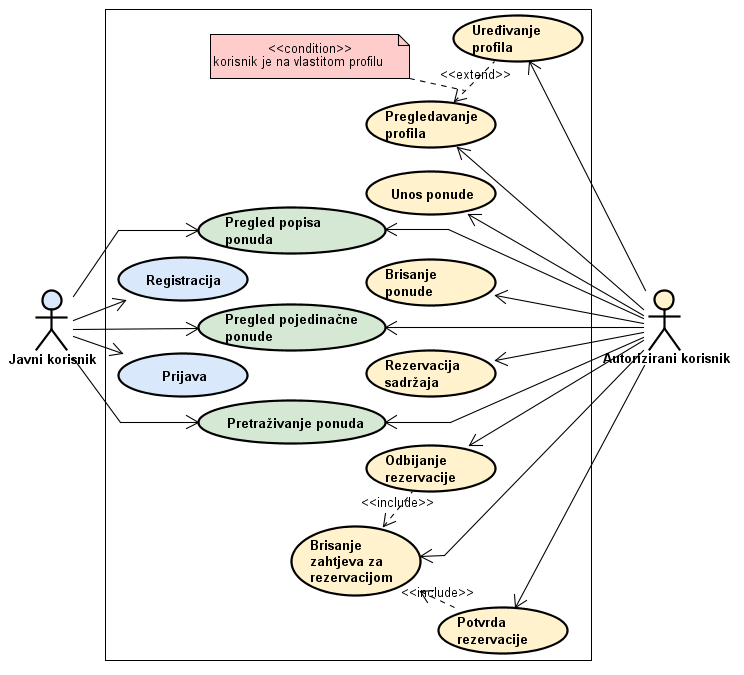
\includegraphics[width=14.7cm]{img/use-case.png}
\caption{Dijagram obrazaca uporabe za funkcionalne zahtjeve korisnika}
\label{fig:use-case}
\end{figure}

\newpage


% Nefunkcionalni zahtjevi
\section{Nefunkcionalni zahtjevi}

Uz navedene funkcionalne zahtjeve korisnika, aplikacija mora također ispuniti sljedeće zahtjeve:

\razmaks
\begin{itemize}
  \item nepredviđena akcija korisnika ne smije uzrokovati prekid rada aplikacije
  \item aplikacija mora raditi u stvarnom vremenu, pri čemu broj korisnika ne smije utjecati na performanse
  \item aplikacija mora biti funkcionalna na svim modernim web preglednicima sa značajnom zastupljenosti na tržištu
  \item funkcionalnosti aplikacije za čije je uspješno izvršavanje potrebna prijava ne smiju biti dostupne bez prijave
  \item navigacija do glavnih dijelova aplikacije mora biti dostupna u svim sučeljima
  \item do glavnih se dijelova aplikacije mora moći pristupiti putem povijesti preglednika
  \item sučelje aplikacije mora biti prilagodljivo za različite veličine ekrana
  \item sučelje ne smije sadržavati autorski sadržaj bez dopuštenja autora
  \item sučelje mora biti napisano na hrvatskom jeziku i podržavati hrvatske znakove
  \item komponente sučelja aplikacije moraju biti građeni prema načelima dobrog oblikovanja kako bi se smanjila međuovisnost i omogućila jednostavna nadogradnja u budućnosti
\end{itemize}


% Implementacija
\chapter{Implementacija}


% Arhitektura i dizajn
\section{Arhitektura i dizajn}

Arhitektura aplikacije temelji se na hijerarhiskoj raspodijeli komponenti.\footnote{Arhitektura temeljena na komponenata \engl{Component-Based Arhitecture} je tipičan način gradnje React aplikacija\citep{understandingCBA}.}
Komponente su odgovorne i znaju samo za one komponente izravno ispod njih u hijerarhiji.
Dvije komponente na odvojenim granama hijerarhije mogu prenositi podatke jedna drugoj ili metodom podizanja stanja\footnote{Vidi pododjeljak \ref{sec:lifting_state}.} ili korištenjem \emph{history} objekta iz \emph{react-router} paketa.
Budući da komponente moraju biti ugnježđene u \emph{Router} komponentu kako bi koristile \emph{history} objekt, takvo prenošenje podataka je ustvari slično podizanju stanja jer također postavljaju stanje roditeljske komponente da bi izazvale promjene. 

Najniže komponente u hijerarhiji enkapsuliraju elemente korisničkog sučelja te idejno ne implementiraju stanje i logiku dalje od toga kako će prikazati podatke.
Glavna ideja iza njih je da budu male i lagane kako bi se mogle ponovno koristiti.
Takve komponente se često nazivaju prezentacijskima i dio gotovih se već nalazi u paketu \emph{react-bootstrap}.

Komponente više u hijerarhiji su zadužene za definiranje stanja i dohvat podataka za niže komponente.
Budući da ove komponente sadrže i definiraju odnos prezentacijskih komponenti, često se za njih koristi izraz \glqq sadržajne komponente\grqq ~ \engl{container components}\citep{componentTypes}.
Ovakve komponente su uglavnom jedinstvene, odnosno teško da će doći do njihovog ponovnog upotrebljavanja.

\newpage


% Raspodjela komponenti
\subsection{Raspodjela komponenti}

Komponente su logički raspodijeljene hijerarhijski s \emph{App} kao najvišom, odnosno korijenskom komponentom.
U nju je izravno ugniježđen \emph{Router} u kojem su definirane sve putanje.
Izvan definicija putanja, no unutar komponente \emph{Router}, je jedino komponenta navigacijske trake (\emph{Navigation}).
Razlog tomu je što se navigacijska traka nalazi u svim dijelovima aplikacije te, budući da je gotovo nepromjenjiva\footnote{Navigacijska traka prikazuje drukčije poveznice ovisno je li korisnik prijavljen u sustav ili ne.}, želi se izbjeći njeno ponovno crtanje pri promjeni putanje.

\razmakp

Ispod navigacijske trake će se, ovisno o putanji, crtati jedna od sljedećih komponenti:
\begin{itemize}
  \item \emph{Main} [\url{/home}] -- glavno sučelje aplikacije
  \item \emph{OfferContainer} [\url{/offer}] -- sučelje u kojem korisnik upravlja vlastitim ponudama
  \item \emph{ReservationContainer} [\url{/reservation}] -- sučelje u kojem korisnik upravlja zahtjevima (primljenim i poslanim)
  \item \emph{ProfileContainer} [\url{/profile/:id}] -- pregled profila korisnika
  \item \emph{ItemDetailsContainer} [\url{/item/:id}] -- pregled detalja ponude
  \item \emph{Login} [\url{/login}] -- obrazac za prijavu
  \item \emph{Registration} [\url{/registration}] -- obrazac za registraciju
\end{itemize}
\razmaks
Svaka od njih, kao i komponenta \emph{Navigation}, definira vlastito stanje i ima pristup \emph{history} objektu\footnote{Vidi odjeljak \ref{sec:react-router}.}.

\razmakp

Daljnje komponente koje definiraju vlastito stanje su \emph{NewOfferForm} i \emph{EditProfileForm}.
One nemaju vlastitu putanju, već su potkomonente od \emph{OfferContainer} i \emph{ProfileContainer}.

Sve ostale komponente aplikacije ne definiraju vlastito stanje.
Potrebne podatke im šalju roditeljske komponente, a sva definirana logika im služi isključivo na prikaz tih podataka.
Primjeri takvih komponenti su \emph{ItemThumbnailContainer}, \emph{ItemThumbnail}, \emph{ItemList}, \emph{ReservationTable}, \emph{ImageColumn} \emph{TextColumn}, \emph{LoadingStatus}, \emph{FieldGroup} i komponente paketa \emph{react-bootstrap}.

\razmakp
\razmakp

Fizički su komponente raspodijeljene svaka u svoju datoteku, koje su potom organizirane u jednu od sljedećih mapa, sukladno obrascima uporabe koje ispunjavaju:
\begin{itemize}
  \item \emph{auth} -- autentifikacija korisnika
    \begin{itemize}
      \item \emph{Login}
      \item \emph{Registration}
    \end{itemize}
  \item \emph{item} -- prikaz ponuda, tj. stvari u ponudama
    \begin{itemize}
      \item \emph{ItemDetailsContainer}
      \item \emph{ItemList}
      \item \emph{ItemThumbnail}
      \item \emph{ItemThumbnailContainer}
    \end{itemize}
  \item \emph{offer} -- upravljanje ponudama
    \begin{itemize}
      \item \emph{NewOfferForm}
      \item \emph{OfferContainer}
    \end{itemize}
  \item \emph{profile} -- prikaz i upravljanje korisničkim podacima
    \begin{itemize}
      \item \emph{EditProfileForm}
      \item \emph{ProfileContainer}
    \end{itemize}
  \item \emph{reservation} -- upravljanje zahtjevima
    \begin{itemize}
      \item \emph{ReservationContainer}
      \item \emph{ReservationTable}
    \end{itemize}
  \item \emph{shared} -- dijeljene prezentacijske komponente
    \begin{itemize}
      \item \emph{ImageColumn}
      \item \emph{LoadingStatus}
      \item \emph{TextColumn}
    \end{itemize}
\end{itemize}
Izvan tih mapa su datoteke s ključnim komponentama aplikacije (\emph{App}, \emph{Navigation} i \emph{Main}) te komponente definirane u vanjskim paketima.

\begin{figure}[htb]
\centering
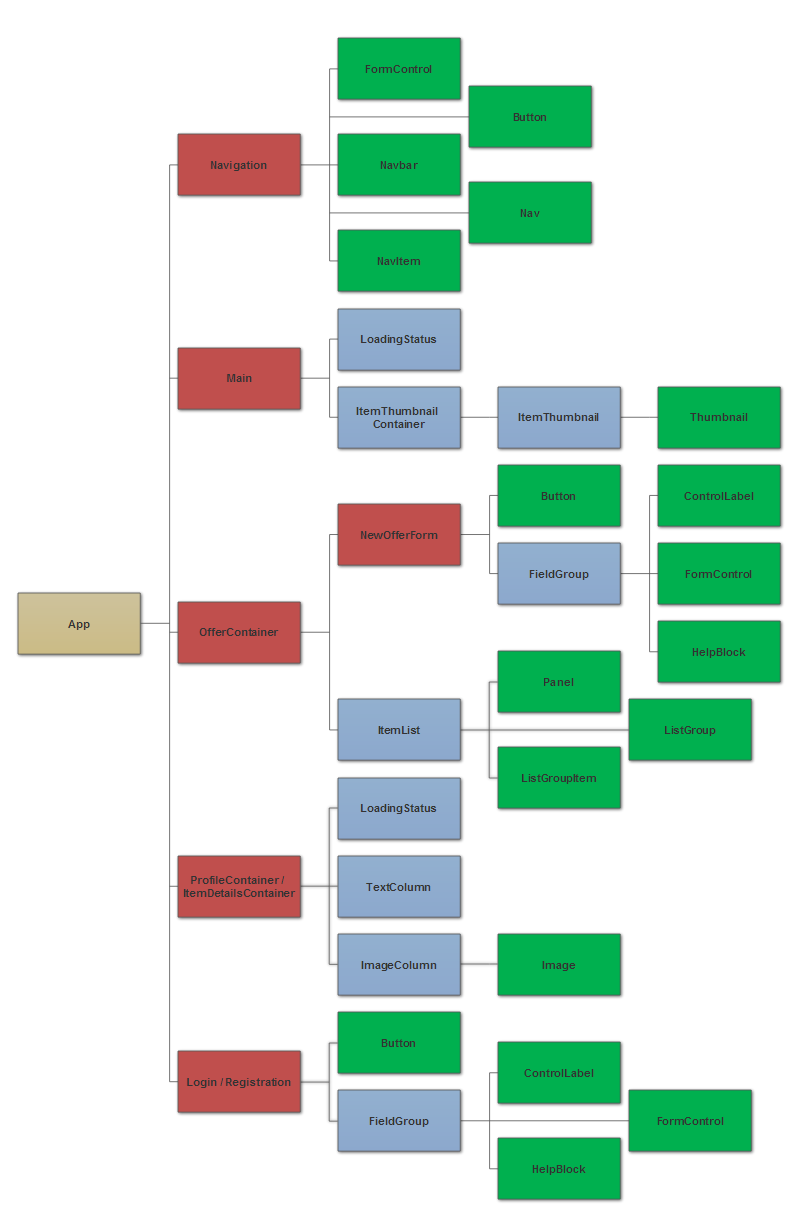
\includegraphics[width=14.5cm]{img/components-tree2.png}
\caption[caption]{Pojednostavljen\footnotemark ~ prikaz hijerarhije komponenti u aplikaciji -- zeleno: komponente iz \emph{react-bootstrap} ; ~ crveno: komponente koje definiraju vlastito stanje}
\label{fig:components-tree}
\end{figure}

\footnotetext{Nedostaje hijerarhija od komponenti \emph{Reservation} i \emph{EditProfileForm} te su komponente koje koriste iste potkomponente grupirane.}

\clearpage


% Pomoćni moduli
\subsection{Pomoćni moduli}

Osim vanjskih biblioteka, komponente koriste pomoćne module za ostvarivanje specifičnih operacija u različitim dijelovima aplikacije.
Dva takva modula su datoteke \emph{Auth.js} i \emph{Constants.js}.

U datoteci \emph{Auth.js} je definirana klasa \emph{Auth} koja sadrži statičke metode koje se koriste za autentifikaciju i autorizaciju korisnika.
Prijavom korisnika u aplikaciju, informacije o korisniku (id i token) spremaju se u \emph{localStorage}\footnote{Objekt za trajno spremanje podataka u pregledniku, svojstvo \emph{Window} objekta. Više na: \url{https://developer.mozilla.org/en-US/docs/Web/API/Window/localStorage}} kako bi se mogle dohvatiti iz različitih komponenti i u različitim instancama aplikacije u istom pregledniku.
Klasa \emph{Auth} definira metode za spremanje, dohvat i brisanje tih informacija.
Ona enkapsulira logiku upravljanja podacima identiteta korisnika što omogućuje jednostavnu izmjenu tih funkcionalnosti.
U slučaju da se u kasnijoj nadogradnji želi preći na neki drugi spremnik, kao što su primjerice kolačići \engl{cookies}\footnote{\url{https://developer.mozilla.org/en-US/docs/Web/HTTP/Cookies}}, potrebno je promjeniti samo kod u datoteci \emph{Auth.js}.

Datoteka \emph{Constants.js} isporučuje nepromjenjive objekte komponentama aplikacije, odnosno služi kao spremnik globalnih konstanti (bez da se stvarno deklariraju u globalnom dosegu).
Jedna takva konstanta je lista kategorija sadržaja (\emph{ITEM\_TYPES}) koja se koristi u komponentama \emph{Main} i \emph{NewOfferForm}.
U prvoj komponenti služi da stvoriti kartičnu navigaciju za filtriranje ponuda\footnote{Vidi slijedeći odjeljak.}, a u drugoj za definirati koje je kategorije sadržaj pri stvaranju ponude.

\newpage


% Glavno sučelje
\section{Glavno sučelje}

Glavno sučelje (na slici \ref{fig:screenshot-main}) je sučelje koje svi korisnici prvo ugledaju kada otvore aplikaciju.
Ono služi za pregled i pronalazak sadržaja, odnosno ponuda, te je jedino sučelje koje u potpunosti nudi iste mogućnosti i javnom i autoriziranom korisniku.
Dapače, jedina razlika u onome što vide javni i autorizirani korisnici je navigacija, koja je ostvarena kao zasebna komponenta (\emph{Navigation}) koja se prikazuje u svim sučeljima aplikacije i mijenja svoj izgled ovisno o tipu korisnika.

\razmaks

\begin{figure}[htb]
\centering
\fbox{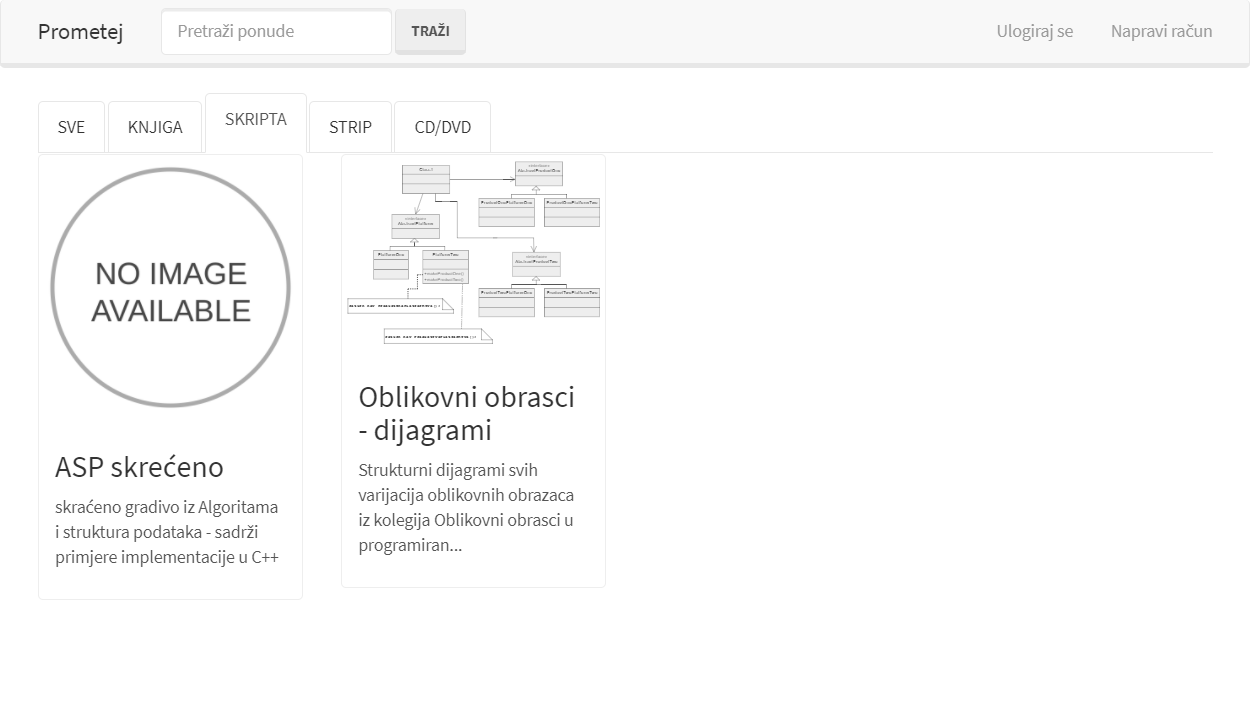
\includegraphics[width=14.2cm]{img/screenshot1_3.png}}
\caption{Glavno sučelje aplikacije}
\label{fig:screenshot-main}
\end{figure}

\razmaks

Izgled sučelja je modeliran pomoću komponente \emph{Main}.
U njoj je definirano stanje, dohvat podataka i navigacija po kategorijama sadržaja pomoću kartica \engl{tabs}.
Također je definirana i logika filtracije sadržaja kojeg šalje kao listu u komponentu \emph{ItemThumbnailContainer}.

Sadržaj se filtrira navigacijom karticama po kategoriji i s obzirom na upit iz tražilice komponente \emph{Navigation}. 
Budući da se tražilica nalazi u navigaciji, komunikacija s komponentom \emph{Main} je ostvarena pomoću \emph{history} objekta, odnosno preusmjeravanjem korisnika na novu rutu.
Upisom teksta u tražilicu korisnika se preusmjerava rutu s upitom (npr. \glqq \url{/home?upit}\grqq ) koja sadrži informaciju o filtraciji.
Potom se filtrira sav sadržaj koji ne sadrži upisani tekst u svom imenu, niti u početku svog opisa.
Filtracija se jednostavno resetira ponovnim klikom na ime aplikacije (u ovom slučaju je radni naslov \emph{Promoetej}) u navigaciji, odnosno odlaskom na rutu \glqq \url{/home}\grqq .

Slanjem liste sadržaja komponenti \emph{ItemThumbnailContainer}, ona stvara potreban broj elemenata komponente \emph{ItemThumbnail}, u kojima je definiran prikaz za elemente liste, te se brine o njihovom razmještaju.
U svakom \emph{ItemThumbnail} elementu je definirana poveznica na \emph{ItemDetails} komponentu za sadržaj kojeg element prikazuje.

\razmakp

Dohvat podataka vrši se u metodi \emph{componentDiDMount}\footnote{Metoda životnog ciklusa komponente. Vidi pododjeljak \ref{sec:components}.} te se podaci spremaju u stanje komponente, što je preporučen obrazac korištenja te metode\citep{reactDocsComponent}.
Dok traje ta operacija, na sučelju crta se komponenta \emph{LoadingStatus} kako bi se korisnika obavijestilo da je dohvat podataka u tijeku.
Ista komponenta crta se i u slučaju greške u dohvatu podataka, samo se korisniku prikazuje poruka da je došlo do greške.

\razmakp
\begin{lstlisting}[language=JavaScript, caption={Metoda \emph{render} komponente \emph{Main}}, label={lst:main_render}]
render() {
  let tabs = ITEM_TYPES.map((type, index) => (
    <Tab eventKey={index+2} title={type.toUpperCase()} />
  ));
  tabs.unshift(<Tab eventKey={1} title="SVE" />);

  return (
    <div>
      <Tabs defaultActiveKey={1}
            onSelect={this.handleSelectCategory}>
        {tabs}
      </Tabs>
      <LoadingStatus isError={this.state.isError}
                     isLoading={this.state.isLoading} />
      <ItemThumbnailContainer items={this.getFilteredItems()} />
    </div>
  );
}
\end{lstlisting}
\razmaks

\newpage


\section{Upravljanje ponudama}

Za upravljanje ponudama su primarno zadužene komponenta \emph{OfferContainer} i njena potkomponenta \emph{NewOfferForm}.
Prva daje pregled svih ponuda koje je korisnik unio u sustav i tuđih sadržaja koje ima u vlasništvu, dok druga služi za dodavanje nove ponude u sustav.
Pristupit im može isključivo autorizirani korisnik klikom u navigaciji na \glqq Vlastite ponude\grqq ~, odnosno na ruti \glqq \url{/offer}\grqq .

\razmaks

\begin{figure}[htb]
\centering
\fbox{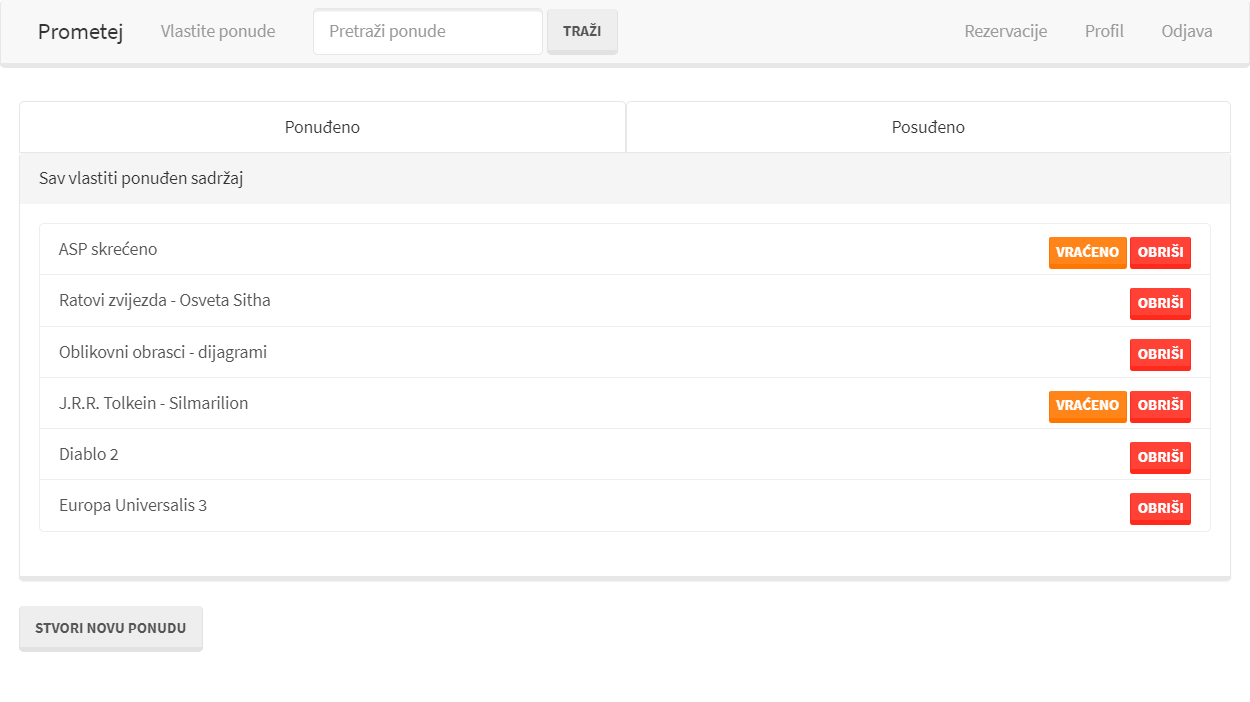
\includegraphics[width=14.2cm]{img/screenshot2_3.png}}
\caption{Sučelje za upravljanje ponudama}
\label{fig:screenshot-main}
\end{figure}

\razmaks

\newpage


\section{Upravljanje zahtjevima}



\chapter{Zaključak}
Zaključak.


% Literatura
\bibliography{literatura}
\bibliographystyle{fer}


% Sažetak
\begin{sazetak}
Tema ovog rada je razvoj korisničke strane aplikacije za razmjenu multimedijskih sadržaja koristeći moderne alate, biblioteke i radna okruženja.
Korisničkog sučelje je izgrađeno korištenjem JavaScript biblioteke React.
Cjelokupna aplikacija korisniku nudi mogućnosti posuđivanja knjiga, stripova, CD-ova, DVD-ova i sl. od drugih korisnika.
Implementira funkcionalnosti: prijave, registracije, dodavanja i upravljanja vlastitog multimedijskog sadržaja, slanje zahtjeva za posuđivanje tuđeg sadržaja, filtrirani pregled svog sadržaja u sustavu.

Cilj rada je ostvarenje jednostavnog i intuitivnog korisničkog sučelja programskog rješenja za razmjenu fizičkih kopija multimedijskog sadržaja te pregled korištenih tehnologija.

\kljucnerijeci{korisničko sučelje, JavaScript, React}
\end{sazetak}

% Abstract
\engtitle{Multimedia Exchange Library User Interface}
\begin{abstract}
The subject of this thesis is the development of a client-side application for a multimedia exchange library using modern front-end tools, libraries and frameworks.
The user interface is built using the React JavaScript library.
The application as a whole enables the user to exchange books, comics, CDs, DVDs, etc. with other users.
The application implements the following functionalities: login, registration, adding and managing owned multimedia items, requesting to borrow other users' items, a filtered overview of all items in the system. 

The goal of this thesis is the realization of a simple and intuitive user interface for a software solution for exchanging physical copies of multimedia items, along with giving an overview of the technologies used in the process.

\keywords{UI, JavaScript, React}
\end{abstract}



\end{document}
